\documentclass[11pt]{article}
\usepackage[left=0.8in,right=0.8in,top=0.7in,bottom=0.7in]{geometry}
\usepackage[numbers]{natbib}
\usepackage{graphicx}
\usepackage{amsmath}
\usepackage{amssymb}
\usepackage[parfill]{parskip} % new line between paragraphs, no indentation
\usepackage[colorlinks,pdfstartview=FitH,citecolor=blue, linkcolor=blue]{hyperref}
\usepackage{xcolor}
\usepackage{xeCJK} % Enabling Chinese characters
\usepackage{mdwlist} % Tight lists
\usepackage{enumerate} % Enabling options for list environments
\usepackage{float}
\usepackage{multirow}
\usepackage{dashrule}
\usepackage[version=4]{mhchem}


% Header
%\usepackage{fancyhdr}
%\pagestyle{fancy}
%\fancyhf{}%Clear all heads and foots
%\setlength{\headheight}{40pt} %Eliminate the warning of "headheight is too samll"
%\rhead{Written Exam Answers\\Jianzhao Bi\\\today}
%\cfoot{\thepage}

% Set font size for "section"
\usepackage{sectsty}
\sectionfont{\fontsize{11}{11}\selectfont}

% Define a new command for text subscript
\newcommand{\tsub}{\textsubscript}

\usepackage{titlesec}
\titlespacing*{\section}{0pt}{0pt}{0pt}

\begin{document}

\setcounter{section}{0}

\section{In a single-sentence, how would you define your research question?}

\section{Missing satellite aerosol optical depth (AOD) data in Aim 1}
\begin{enumerate*}[{[a)]}]
    \item For the AOD over land surfaces, the major causes of missing data include (1) cloud cover, (2) snow/ice cover, (3) inland water bodies, and (4) no measurement (\textit{i.e.,} data points outside the satellite scanning range). These sources led to different proportions of missing data. Take New York State in 2015 as an example, the cloud-cover, snow-cover, no measurement, and inland water led to $\sim$75\%, $\sim$6\% (it increased to $\sim$20\% in the snow season), $\sim$10\%, and $< 1\%$ of missing AOD data, respectively. 
    
    The AOD observation could not be conducted in desert and semidesert regions by the original aerosol retrieval algorithm -- Dark Target (DT) \citep{kaufman1997modis, levy2007second}, because it was difficult to separate the aerosol signal from the top-of-atmosphere (TOA) reflectances at red and near-infrared wavelengths \citep{hsu2013enhanced}. Currently, a new algorithm -- Deep Blue (DB) \citep{hsu2004aerosol} utilizes blue wavelength where the surface reflectnace over land is much lower than for longer wavelength channels (\textit{i.e.,} red and near-infrared wavelengths). DB has successfully produced aerosol products over desert and semidesert areas and expanded the AOD availability to all cloud-free and snow/water-free land surfaces \citep{hsu2013enhanced}. 
    
    Major strategies dealing with the issue of missing AOD data can be classified as four categories. The first strategy is to adjust and improve current aerosol retrieval algorithms to increase available AOD estimations \citep{van2011satellite}. The second one is to utilize the spatiotemporal autocorrelation of AOD/PM\tsub{2.5} to interpolate the missing data by geostatistical interpolation approaches (\textit{e.g.,} universal kriging) \citep{kloog2011assessing, kloog2012incorporating}. The third one is using simulated AOD by chemical transport models in the regions without AOD measurements \citep{hu2017estimating}. The fourth one is to regress the missing AOD by statistical/machine learning models with AOD-related physical and land-use parameters (\textit{e.g.,} cloud fraction, meteorological parameters, elevation, \textit{etc.}) \citep{xiao2017full}.
    
    \item In my opinion, the biggest concern comes from the non-random nature of the missingness. It has been found that cloud and snow can lead to the change of AOD levels because of the shifted AOD physical characteristics under different meteorological conditions \citep{alam2014variability, kang2015correlation, emili2011high}. Thus, it may induce potential biases when missing AOD data are estimated only from existing AOD observations or under an incomplete consideration of the associations between cloud/snow and AOD. Considering the 90\% of missingness, this large proportion of potentially biased estimations might then affect the precision of PM\tsub{2.5} prediction in terms of its values and spatiotemporal patterns. For the health analyses, the measurement error of PM\tsub{2.5} can then lead to bias toward the null in estimated associations between PM\tsub{2.5} and its health outcomes \citep{sarnat2015fine}, that is, the underestimation of the adverse health effect of PM\tsub{2.5}.
    
    \item In this study, we are trying to reduce the systematic bias caused by the non-random missingness by incorporating AOD-related cloud/snow parameters in an appropriate statistical or machine learning model. For one thing, according to the validation of gap-filled AOD by the preciser ground-based AOD observations (\textit{i.e.,} AERONET data), utilizing the parameters relating to the cloud-/snow-AOD interactions (\textit{e.g.,} cloud/snow fractions) has been proven to be an effective way to estimate the systematic change of AOD levels and increase the precision of AOD estimation \citep{xiao2017full}. For another, an appropriate regression model is also key to an accurate gap-filling since the relationships between AOD and meteorological parameters are complex. The preliminary analysis of this study has shown that machine learning models (\textit{e.g.,} Random Forests and Neural Networks) performed much better than the multiple imputation model \citep{xiao2017full} which is a latest statistical model used in AOD gap-filling. This comparison indicates the advantage and potential of machine learning models dealing with complex interactions which can hardly be described by current statistical models. Admittedly, our current consideration about possible parameters explaining the cloud-/snow-AOD interactions is still limited and incomplete, and thus the bias will still exist in the AOD estimations. We will further examine more cloud/snow parameters and try to more precisely recover the relationships between cloud/snow and AOD.
\end{enumerate*}

\section{Low-cost sensor observations for \texorpdfstring{PM\tsub{2.5}}{PM2.5} predictions in Aim 2}
\begin{enumerate*}[{[a)]}]
    \item Yes. Based on some previous studies \citep{hu2017estimating, di2016assessing} and the preliminary results of this study, the convolutional layer of PM\tsub{2.5} measurements (applying a convolution kernel, here is an inverse distance weighting (IDW) kernel, on the input layer), as an additional predictor variable to account for spatial autocorrelation of PM\tsub{2.5}, has a larger contribution to the PM\tsub{2.5} predictions than satellite AOD data in the prediction models, and can significantly improve the model performance. Specifically, both \citet{hu2017estimating} and the preliminary analysis of this study showed that the PM\tsub{2.5} convolutional layers had the highest variable importance values in the PM\tsub{2.5} models based on the random forest algorithm. Similarly, in Equation 4 of the proposal, we are planning to produce a convolutional layer for low-cost sensor measurements which have a larger density than the regulatory stations, so it is expected to provide more detailed spatial patterns of PM\tsub{2.5} and have a significant contribution to the model performance. 
    
    \item Even though the PM\tsub{2.5} convolutional layer has greater influence and importance than satellite AOD in terms of the model performance, it cannot be said that satellite AOD is less important in the process of PM\tsub{2.5} estimation. The indicator of the model performance -- cross-validation -- can only be conducted in the areas with regulatory PM\tsub{2.5} stations, and these stations are currently unevenly distributed and only accumulated in the populated areas. Therefore, the model performance is unknown in the areas without regulatory stations, such as some rural areas and wild areas. As a result, it cannot be directly extrapolated that the PM\tsub{2.5} convolution is more important than the satellite data in these regions. In fact, since the satellite scans the land surfaces in the same way, unlike the PM\tsub{2.5} convolutional layer, it can provide a more stable data quality in both urban and rural areas. 
    
    Further, in order to assess the contribution of satellite AOD to the PM\tsub{2.5} predictions, we built a no-AOD prediction model in the preliminary analysis of this study. Figure \ref{fig:noaod} shows the spatial differences between full-model and no-AOD PM\tsub{2.5} in the snow season of 2015 (first 15 weeks). Compared to the no-AOD PM2.5, the full-model PM2.5 had changes in the spatial pattern with intensified on-road emissions. Hence, the pollution information provided by the satellite AOD can influence the PM\tsub{2.5} predictions in a discernible way. 
    
    \item If I had funds to invest in future data collection, I recommend first applying for the quality improvement of low-cost sensors, and then applying for the denser deployment of low-cost sensors, and finally applying for the development of new satellite sensors. In my opinion, this route can provide the quickest and most direct improvement for the PM\tsub{2.5} exposure assessment. Because of the smaller size and inexpensive deployment cost, the low-cost continuous monitoring instruments can potentially fill in gaps in the regulatory monitoring network to enhance the understanding of pollution hotspots \citep{gao2015distributed}. However, their large measurement errors hinder a wider application of them to assess compliance with air pollution standards \citep{hall2014integrating}. Once the low-cost sensors have reliable measurement qualities, it will be much easier to densely employ them to cover all population than the regulatory stations, and it might become the new ``regulatory'' measurements with high spatiotemporal coverage. Satellite sensors cannot provide direct obsevations of PM\tsub{2.5} so far, which limits their capability in PM\tsub{2.5} exposure assessment. However, satellite remote sensing can provide global-scale observation and are important to pollution event detection, transport and model prediction, and emission estimation \citep{hoff2009remote}, which are the unique advantages over the ground measurements. Consequently, satellite data are still valuable complements to the ground measurements, and with its evolving functions, it will play more important roles in the fields of environment and public health. 
\end{enumerate*}

\section{In your words, describe the specific parameter selection strategy for Equation 2}

\hdashrule{\textwidth}{0.1pt}{3mm 3pt 1mm 3pt}
\setcounter{section}{0}

\section{How generalizable do you anticipate the \texorpdfstring{PM\tsub{2.5}}{PM2.5} models in Aims 1 and 2 to be?}
\begin{enumerate*}[{[a)]}]
    \item For the AOD gap-filling model (Equation 1), PM\tsub{2.5} prediction model (Equations 2), and PM\tsub{2.5} interpolation model (Equation 3), the generalizability mainly depends on the qualities of input data (\textit{i.e.,} satellite observations, regulatory measurements, meteorological data, and land-use data). In the United States, these datasets are well generated, validated, organized, and maintained, so they have good and stable data qualities. As a result, it is expected that these models are generalizable in the US. In fact, several studies \citep{kloog2011assessing, kloog2012incorporating, hu2017estimating, di2016assessing} have utilized similar models and datasets at regional and national scales in the US, generating high-resolution PM\tsub{2.5} predictions with good model performance. Further, the preliminary analysis of this study also applied these models in Imperial County, California, obtaining PM\tsub{2.5} predictions with similar performance as which in New York State. 
    
    For the PM\tsub{2.5} prediction model with low-cost sensor measurements (Equation 4), apart from the qualities of above-mentioned datasets, the availability of low-cost sensors is also key to the generalizability of the model. Figure \ref{fig:pa} shows the current distribution of PurpleAir low-cost monitors in the United States. According to the figure, the densest PurpleAir networks are on the west coast, especially in California, and in some eastern states, such as New York State, Pennsylvania, Maryland, North Carolina, \textit{etc.} For a regional-scale study, Equation 4 is expected to be generalizable to these states with dense PurpleAir networks. However, similar studies can only be conducted at local scales (such as county-level or city-level) in which there are limited low-cost sensors. 
    
    For the low-cost sensor calibration models (Equations 5 and 6), the generalizability should be further examined since no similar study has been conducted using these models for a nationwide, or even a statewide, low-cost sensor network. \citet{carvlin2017development} has calibrated Dylos PM sensors (Dylos Corporation, Riverside, CA) by regulatory measurements in Imperial County, California, showing that the measurement quality of the sensors is associated with meteorological conditions such as temperature and relative humidity. Studies \citep{broday2017wireless, castell2017can} also showed that the quality of laser-based PM\tsub{2.5} sensors is associated with particle size and PM composition. Therefore, our calibration models should be carefully tested, and adjusted if necessary, before generalize to other areas. 
    
    \item The limitation of generalizing Equations 1 -- 4 elsewhere mainly comes from the qualities of input data. In the areas with reliable input data, the PM\tsub{2.5} prediction is expected to be effectively conducted. For example, \citet{xiao2017full} used similar input datasets to estimate missing satellite AOD and PM\tsub{2.5} concentrations in Yangtze River Delta (YRD) of China in 2013 and 2014, which had good model performance with cross-validation R$^2$s of $\sim$0.8. In contrast, the preliminary analysis of this study used the same models in Lima, Peru to estimate PM\tsub{2.5} concentrations, but obtaining significantly worse model performance because of the lack of necessary data and limited data qualities and quantities. In order to maximize the prediction ability in this situation, the datasets should be carefully selected and the models should also be properly adjusted.
    
    The limitation of generalizing Equations 5 -- 6 mainly comes from the characteristics of specific low-cost sensors. For example, PM composition, relative humidity, and temperature may affect the precision of a sensor \citep{carvlin2017development, broday2017wireless, castell2017can}. The non-linear response to the PM\tsub{2.5} concentrations \citep{kelly2017ambient} and the quality degredation \citep{broday2017wireless} may also lead to the measurement errors. Thus, before applying to other regions, the calibration models should be examined, and then be adjusted according to the examination, such as adding appropriate covariates. 
\end{enumerate*}

\section{What factors might you be concerned about before using PurpleAir data?}
The most important factor having to be concerned about before using the data of the PurpleAir monitoring network is the quality of the PM\tsub{2.5} measurements. The methods of PM\tsub{2.5} measurement used in regulatory monitors are Federal Reference Method (FRM) or Federal Equivalent Method (FEM). This indicates that they have been developed to a clearly defined standard for PM\tsub{2.5} and have completed a rigorous testing and analysis protocol before they can be used to monitor compliance for the appropriate primary and/or secondary National Ambient Air Quality Standards (NAAQS) \citep{hall2014integrating}. On the contrary, no standard or protocol has been established for the newly emerged low-cost sensors, so their qualities cannot be guaranteed to assess compliance for NAAQS. For example, The maximum consistency errors of PurpleAir sensors (PA-II: Dual Laser Air Sensors) are $\pm$10\% in the range of 100 -- 500 $\mu g/m^3$ and $\pm$10 $\mu g/m^3$ in the range of 0 --100 $\mu g/m^3$. In this study, we plan to use two strategies to minimize the adverse effect of the low quality of PurpleAir sensors and to incorporate their measurements in the PM\tsub{2.5} prediction models:
\begin{enumerate*}[{[1)]}]
    \item \textbf{Using PurpleAir measurements as a predictor variable}: In the benchmark approach of Aim 2, we will use the interpolated PurpleAir PM\tsub{2.5} measurements (by Equation 3) as a predictor variable in the PM\tsub{2.5} prediction model (Equation 4). This approach will not only utilize the spatial details of the measurements but also reduce the adverse effects of the measurement errors on the regression stage of the model. However, this approach will not increase the sample size of the dependent variable, so the model performance will still be limited if there are not enough regulatory PM\tsub{2.5} observations in the study domain. 
    \item \textbf{Calibrating and utilizing the measurements as the dependent variable}: In order to increase the sample size of the dependent variable and fully utilizing the spatial details of the PurpleAir measurements, we plan to calibrate these data by the regulatory observations. The difficulties include the determination of an appropriate ``collocated'' distance between a PurpleAir sensor and the regulatory stations and the reliable extrapolation of the calibration coefficients. For the former problem, we will examine a series of distances and choose the most suitable one by cross-validation of the calibration model. For another problem, apart from the proposed kriging with external drift (KED) model, we will also test other interpolation methods (such as variational interpolation \citep{turk1999shape}) to obtain reasonable spatial representations of the calibration coefficients. 
\end{enumerate*}

\section{How you will determine whether or not given \texorpdfstring{PM\tsub{2.5}}{PM2.5} exposures are ``reliable''?}
In this study, the ``reliability'' of PM\tsub{2.5} exposures is defined from three aspects: (1) spatiotemporal completeness, (2) statistical reliability, and (3) improvement of actual reliability in populated areas.
\begin{enumerate*}[{[1)]}]
    \item First, our PM\tsub{2.5} exposure dataset has 1-km, daily resolutions with complete coverage in space and time. In general, the routine measurements made by local and federal monitoring programs cannot provide continuous, daily availability, which limits their usefulness for studies of associations between health outcomes and daily variations in pollutant concentrations \citep{sarnat2015fine}. On the contrary, the spatiotemporal completeness enables the application of our exposure dataset to the health analyses of associations between health outcomes and short-term pollution exposure. 
    \item In addition, the good statistical performance of our prediction models is an important standard to assess the reliability of the exposure dataset. We will use cross-validations (CV) as the evaluation method of model performance. This method involves partitioning the input data into complementary subsets, performing the analysis on one subset (called the \textit{training set}), and validating the analysis on the other subset (called the \textit{validation set} or \textit{testing set}) \citep{kohavi1995study}. It aims to test the model's ability to predict new data that were not used in estimating it, rather than the model fitting ability, in order to avoid the problem of overfitting \citep{hawkins2004problem}. Similar studies using statistical models \citep{kloog2011assessing, kloog2014new} and machine learning models \citep{di2016assessing, hu2017estimating} obtain PM\tsub{2.5} predictions with CV R$^2$ of $\sim$0.8 and root-mean-square error (RMSE) of $\sim$3 $\mu g/m^3$. The preliminary results of this study showed that our prediction models are expected to have similar or even better statistical performance than the previous studies. 
    \item Admittedly, good statistical performance does not necessarily mean good actual performance. Specifically, the cross-validation can only evaluate the actual model performance in the areas with regulatory stations, such as cities and populated areas. In other words, the model performance is unknown in the areas without regulatory stations, such as wild areas. However, since our goal is to analyze the health effect of PM\tsub{2.5} on the population, the unknown data quality in wild areas, where there are few populations exposing to the pollutant, are expected to have less influence on our estimated health effects. Moreover, the low-cost sensors will further fill in the gaps of regulatory stations, providing more spatial details of local pollution levels in populated areas. With high cross-validation performance and the supplementation of low-cost sensors, our prediction models are expected to guarantee the actual reliability of exposure assessment for the majority of population exposing to PM\tsub{2.5} pollution. 
\end{enumerate*}

\section{Temporal and spatial misalignment among the proposed data sources}
\begin{enumerate*}[{[a)]}]
    \item Table \ref{tab:res} shows the spatial and temporal resolutions of the data sources used in this study, including satellite/chemical transport model (CTM) data, meteorological data, land-use data, and point data (PM\tsub{2.5} emissions and concentrations). 
    \item All datasets with different spatial and temporal resolutions will be matched and integrated into the 1-km, daily grid of MAIAC AOD. All models in Aims 1 and 2 will also be based on this grid. {
        \begin{itemize*}
            \item \textbf{Spatial integration}: For the datasets with spatial resolutions greater than or equal to 1-km (\textit{e.g.,} CMAQ simulations, meteorological data, and MODIS cloud/snow parameters), geostatistical interpolations (inverse distance weighting \citep{bartier1996multivariate} or kriging interpolation \citep{oliver1990kriging}) will be applied. For the datasets with finer resolutions (\textit{e.g.,} ASTER elevation and MODIS NDVI), a simple down-sampling process will be conducted. For the LandScan population, each data point will be assigned to its nearest MAIAC grid cell. The population of all points falling in that grid cell will then be summarized. For the point datasets (\textit{e.g.,} NEI PM\tsub{2.5} emissions, EPA, NAPS, and PurpleAir PM\tsub{2.5} measurements), each monitoring site will be assigned to the MAIAC grid cell where it is located. The average PM\tsub{2.5} will be calculated when multiple points fall in the same grid cell. 
            \item \textbf{Temporal integration}: For the datasets with temporal resolutions less than 1 day (\textit{e.g.,} MAIAC AOD, CMAQ simulations, MODIS cloud/snow parameters, meteorological data, and PM\tsub{2.5} ground measurements), daily average values will be calculated. For MODIS NDVI, the 16-day average NDVI values will be replicated in each day of this period. The land-use data and NEI PM\tsub{2.5} emissions can be treated as temporally invariant in the annual PM\tsub{2.5} prediction models. 
        \end{itemize*}
    \item For the spatial integration, major assumptions come from the oversampling processes (\textit{i.e.,} geostatistical interpolations). For example, the inverse distance weighting (IDW) is based on an assumption that the value at an unsampled point can be approximated as a weighted average of values at points within a certain cut-off distance, or from a given number of the closest points \citep{bartier1996multivariate}; Kriging interpolation is based on a concept of random functions: the values in a surface are assumed to be the realizations of a random function with a certain spatial co-variance \citep{oliver1990kriging}. Each of the interpolation methods has limited applicability. Therefore, careful examination and proper choice of the method and its parameters for each dataset are important to avoid misalignment and improve the final results \citep{mitas1999spatial}.
    
    For the temporal integration, major assumptions come from the temporal invariability of some parameters. For example, we assume that the study domain has similar NDVI values in a 16-day period; we also assume that other land-use parameters (elevation, population, and road network) are stable in a year. Even though these assumptions may induce potential errors, these errors are expected to have much less influence than the major sources of error (such as inaccurate measurements and model misspecification) \citep{xiao2017full}.
    }
\end{enumerate*}

\hdashrule{\textwidth}{0.1pt}{3mm 3pt 1mm 3pt}
\setcounter{section}{0}

\section{How could short-term exposure to \texorpdfstring{PM\tsub{2.5}}{PM2.5} cause acute kidney problems?}
Acute renal failure (ARF) is an abrupt loss of kidney function that develops within 7 days. Generally, it occurs because of damage to the kidney tissue caused by decreased kidney blood flow (kidney ischemia) from any cause (\textit{e.g.,} low blood pressure), exposure to substances harmful to the kidney, an inflammatory process in the kidney, or an obstruction of the urinary tract that impedes the flow of urine. Interest in the nonpulmonary targets of particulate air pollutants has been increasing since the demonstration that inhaled ultrafine particles (UFP) can affect distant organs either by direct passage across the alveolar capillary barrier and/or by the release of soluble inflammatory mediators and markers of oxidative stress into the systemic circulation, which may affect several distant organs including the kidney \citep{nemmar2004possible, oberdorster2005nanotoxicology, peters2006translocation, vermylen2005ambient, nemmar2013recent}. 

It is hypothesized that renal function impairment may be a mediating factor of the cardiovascular effects of PM\tsub{2.5} exposure because the kidney is a vascularized organ susceptible to large-vessel atherosclerotic disease and microvascular dysfunction \citep{lue2013residential}. Three distinct hypotheses have been proposed to explain the epidemiologic observations of a relationship between PM2.5 and cardiovascular outcomes; these may also be pertinent in the evaluation of renal outcomes \citep{bowe2018particulate}:
\begin{enumerate*}[{[1)]}]
    \item Inhaled particles provoke pulmonary inflammation which may then lead to systemic inflammation \citep{chin2014basic}, including kidney. 
    \item The mechanism involves pollutant-induced disturbances in the lung autonomic nervous system \citep{chin2014basic}. Specifically, the inhalation of particles may trigger a reflex that leads to a subtle change in the rhythm of the heart. When the heart is no longer pumping efficiently it becomes congested with blood, causing pressure to build up in the main vein connected to the kidneys and leading to congestion of blood in the kidneys. The kidneys also suffer from the reduced supply of oxygenated blood \citep{kazory2009anemia}. 
    \item Air-borne particulates enter the bloodstream where they may then interact with tissue components to promote the observed pathologic effects. This is supported by emerging evidence suggesting that inhaled inert gold nanoparticles not only enter the bloodstream of healthy adult volunteers, but are detected in the urine within minutes after exposure, providing a proof of concept that inhaled nanoparticles get filtered and excreted by the kidney \citep{chin2014basic, miller2017inhaled}.
\end{enumerate*}
Furthermore, it is plausible that one or more of the following mechanistic pathways may explain the aforementioned hypotheses regarding the association between the exposure to PM\tsub{2.5} and kidney disease:
\begin{enumerate*}[{[1)]}]
    \item Increased inflammatory mediators (including TNF-$\alpha$, IL-6, and PAI-1), oxidative stress \citep{ostro2014chronic, ruckerl2014associations, sorensen2003personal}, increased atherosclerotic plaque area, and exaggerated vasoconstrictor responses to phenylephrine and serotonin \citep{sun2005long}.
    \item Significant decrease in flow-mediated dilatation \citep{krishnan2012vascular, wilker2014relation}, increases in systolic BP and pulse pressure \citep{auchincloss2008associations, fuks2014arterial, fuks2011long}, and disturbances in the hypothalamic-pituitary-adrenal axis \citep{thomson2013mapping}.
    \item  Metabolic disturbances, including glucose intolerance, decreased insulin sensitivity, higher blood lipid concentrations, weight gain, and increased risk of diabetes mellitus \citep{wei2016chronic, chen2016ambient, wolf2016association}.
\end{enumerate*}

\section{Heterogeneity of exposure-health outcome results across cities or states}
\begin{enumerate*}[{[1)]}]
    \item \textbf{Sample size}: Different cities may have different sample sizes (in this case, the number of emergency department visits). A small sample size can lead to a less power of the model and a larger confident interval of the estimated effect, which would increase the uncertainty of the result. In addition, a small sample size would also lead to selection bias, that is, the study population is meaningfully different from the source population. This would also induce large errors to the estimated effect, leading to heterogeneity in results across individual cities. 
    \item \textbf{Socioeconomic characteristics}: Populations in different cities may have different distributions of socioeconomic characteristics, which would be the potential effect modifiers of the associations between PM\tsub{2.5} exposure and renal outcomes. These characteristics include age, sex, race, education level, income level, marital status, occupation, religion, birth rate, death rate, average size of a family, average age at marriage, \textit{etc.} Specifically, \citet{janssen2002air} and \citet{medina2006effect} found that the proportion of central air conditioning modified the effect of PM\tsub{10} on hospital admissions for cardiorespiratory disease, a possible reason for which might be the lower ventilation rates of homes with air conditioning \citep{suh1992personal}. 
    \item \textbf{PM\tsub{2.5} sources}: The same PM\tsub{2.5} component may come from different sources. For example, secondary sulfate (\ce{SO^{2-}_4}) can be generated from sulfur dioxide (\ce{SO2}) emissions from power plants, industrial facilities, and traffic sources. Particulate matters from different sources may have different levels of health effects. For example, studies \citep{laden2000association, zeka2005short} found that PM\tsub{10} and PM\tsub{2.5} from mobile sources were associated with a higher mortality risk than particulate matters from other sources. the There is also evidence that the hazardous nature of combustion-related PM (from both mobile and stationary sources) is more consistent than that for PM from other sources \citep{world2007health}.
    \item \textbf{Synergy effect of gaseous pollutants}: Gaseous pollutants have health effects of their own and may act in concert with PM to cause health effects (\textit{e.g.,} ozone). Any consideration of the health effects of different components and sources of PM must consider how gaseous pollutants may affect the toxicity of PM constituents \citep{adams2015particulate}.
    \item \textbf{Other potential confounders}: Some well-understand confounders, such as season, day of week, holidays, temperatures, and time trends, will be selected \textit{a priori} as the covariates in our time-series model. However, there may still be other potential confounders affecting the relationship between PM\tsub{2.5} exposure and renal disease, leading to heterogeneity in results across individual cities. 
\end{enumerate*}

\section{Measurement errors in the \texorpdfstring{PM\tsub{2.5}}{PM2.5} estimates and the ED visit data}
\begin{enumerate*}[{[a)]}]
    \item The measurement errors of satellite aerosol optical depth (AOD) can come from the receiving of raw signals and the retrieval process. The random and/or systematic biases of the satellite sensors and other atmospheric and geometric interference may induce errors in raw signals. After recording raw signals, AOD will be estimated by specific algorithms (also called ``retrieval''). This process will also induce some errors due to the reliability of algorithms and other input data. 
    
    The regulatory PM\tsub{2.5} measurements (\textit{e.g.,} EPA AQS measurements) are always treated as the ``gold standard'' of PM\tsub{2.5} concentrations since they have been developed to a clearly defined standard for PM\tsub{2.5} and have completed a rigorous testing and analysis protocol before they can be used to monitor compliance for the air quality standards \citep{hall2014integrating}. However, their measurements may not always represent the pollution level in its surrounding area because they may be affected by short-term pollution events (\textit{e.g.,} heating, ventilation, obstruction \textit{etc.}) in their nearby microenvironments \citep{carvlin2017development}. This is a kind of regulatory monitor's ``measurement error''.
    
    Most of the current low-cost sensors (including PurpleAir) use laser reflections to count particles in the air, and then these particle counts are processed by the sensors to calculate the PM\tsub{2.5} mass. The measurement errors can come from these two processes. First, the particle counts may have a relatively large inaccuracy \citep{northcross2013low}. In addition, the conversion from particle counts to particle mass may also be affected by some factors, such as PM composition, temperature, and relative humidity \citep{ gao2015distributed, carvlin2017development}, leading to additional errors. Moreover, as the regulatory monitors, the low-cost sensors may also suffer from the short-term pollution events in nearby microenvironments, thus having less representativeness of their surrounding pollution levels. 
    
    For the emergency department (ED) visit data, inaccurate coding is a major source of measurement error. For example, kidney disease tends not to be coded as primary diagnosis even though sometime it may be a major but potential reason for the admission. In addition, incorrect diagnosis is also a possible reason for the measurement error in ED visit data. 
    
    \item All of the aforementioned measurement errors can be referred to as ``misclassification'', and all of them can affect the results from the health impact analysis. The measurement errors of satellite and ground monitors are the misclassification of exposure, and the measurement errors of ED visit data are the misclassification of disease. Since the misclassification of PM\tsub{2.5} exposure is the same for those with renal disease as it is for those without renal disease, this kind of misclassification is non-differential and the bias of the health effect tends to be towards the null \citep{sarnat2015fine}. Similarly, the pollution level is in general not associated with the diagnosis accuracy of doctors, so the misclassification of outcome may also be non-differential, that is, the bias tends to be towards the null as well. Overall, the measurement errors of PM\tsub{2.5} monitors and ED visit data can generally lead to the underestimation of the adverse health effect of PM\tsub{2.5}.
    
    \item An ideal PM\tsub{2.5} exposure dataset should include: {
        \begin{itemize*}
            \item \textbf{Pollutant sources}: Where are the PM\tsub{2.5} coming from, at what rate? What are the indoor and outdoor PM\tsub{2.5} concentrations? What is the composition of these particulate matters?
            \item \textbf{Population of concern}: Who are the individuals that are exposed? How are the factors of the population relating to the dose of pollutant (\textit{e.g.,} age, sex, body weight, \textit{etc.})? 
            \item \textbf{Exposure pathways}: Through which pathways is the population exposed to PM\tsub{2.5}? What proportion of PM\tsub{2.5} is exposed through inhalation?
            \item \textbf{Activity patterns}: How much time the population stay indoor and outdoor? What are the population's exposure duration and frequency? 
            \item \textbf{Inhalation rates}: What are the inhalation rates of the population according to the age, sex and activity pattern?
        \end{itemize*}
    }
\end{enumerate*}

\section{Benefits and limitations of the direct measurement of individual exposure}
\begin{itemize*}
    \item Benefits {
        \begin{enumerate*}[{[(1)]}]
            \item Direct personal monitoring is the most accurate means of exposure assessment. Regulatory measurements are subject to biases because most people spend much more of their time indoors than out, and air pollutant concentrations are often much higher inside buildings than outside \citep{spengler1983indoor}. In addition, the time people spend in different locations and their activities vary dramatically with age, gender, occupation, and socioeconomic status, causing difficulty in adequately characterize the pollutants they are exposed to. In contrast, a personal exposure depends on the air pollutant concentrations that are present in the locations the person moves through as well as on the time spent in each location. This approach allows the exposure assessment for a specified group of people with widely different time-activity patterns \citep{watson1988air}. 
            \item The health effect study at the individual-level is able to more precisely reflect the association between PM\tsub{2.5} exposure and ED visit for kidney disease. In the case of region/community-level study, it is unknown that if the patients visiting the emergency department have indeed been exposed to high-level PM\tsub{2.5}. It is possible that the higher-level PM\tsub{2.5} pollution is accidentally associated with an increased number of ED visit for renal disease. On the contrary, individual-level study will establish a more powerful causal link between the individually experienced PM\tsub{2.5} levels and ED visits.
            \item If study participants maintain records of their activities, then locations where highest concentrations occur as well as the nature of emission sources can often be inferred. This is a helpful reference for the community to reasonably deploy regulatory air quality monitoring stations \citep{watson1988air}.  
        \end{enumerate*}
    }
    \item Limitations {
        \begin{enumerate*}[{[(1)]}]
            \item Personal monitoring studies are complex, expensive, time-consuming, and labor-intensive. Compared to the community-level study, it is more difficult to recruit larger populations in a wider area to conduct similar analyses, which can significantly limit the power and the generalizability of the study. 
            \item It tends to have problems regarding the selection and recruitment of representative subjects. Personal exposure monitoring is an intrusive event in the life of the study participants. The demands of the project protocol and the associated inconvenience may cause many people to refuse to cooperate, leading to high dropout rates. In addition, it is particularly difficult to get the cooperation of schoolchildren, non-native speakers, disadvantaged people, or those with low socioeconomic status \citep{watson1988air}. These problems may lead to the selection bias in the study population and affect the generalizability of the estimated health effects. 
            \item Wearing a monitor or filling out a log can cause the participant to change his or her behavior and consequently introduce more biases in the estimated effects \citep{ryan1986estimating}.
        \end{enumerate*}
    }
\end{itemize*}

% ----------- Figures & Tables ----------- %
\newpage
\begin{table}[H]
    \centering
    \caption{Spatial and temporal resolutions of the data sources}
    \begin{tabular}{c|c|c|c}
        \hline
        \multicolumn{2}{c|}{Data Source} & Spatial Resolution & Temporal Resolution \\
        \hline
        \multirow{2}{*}{Satellite/CTM} & MAIAC AOD & 1 km & $<$ 1 day \\
        & CMAQ Simulation & 12 km & 1 hour \\
        \hline
        \multirow{4}{*}{Meteorology} & MODIS Cloud & 1 km & $<$ 1 day \\
        & MODIS Snow & 0.05$^{\circ}$ ($\sim$ 5 km) & $<$ 1 day \\
        & NARR & 0.25$^{\circ}$ ($\sim$ 25 km) & 3 hours\\
        & NLDAS & 0.125$^{\circ}$ ($\sim$ 13 km) & 1 hour \\
        \hline
        \multirow{4}{*}{Land-Use} & ASTER Elevation & 1$^{\prime\prime}$ ($\sim$ 30 m) & -- \\
        & LandScan Population & 900 m & 1 year \\
        & MODIS NDVI & 500 m & 16 days \\
        & ESRI Road Network (vector) & -- & 1 year \\
        \hline
        \multirow{3}{*}{Point Data} & NEI PM\tsub{2.5} Emissions  & -- & 3 years \\
        & EPA/NAPS PM\tsub{2.5} & -- & 1 day \\
        & PrupleAir PM\tsub{2.5} & -- & $<$ 1 hour \\
        \hline
    \end{tabular}
    \label{tab:res}
\end{table}

\begin{figure}[H]
    \centering
    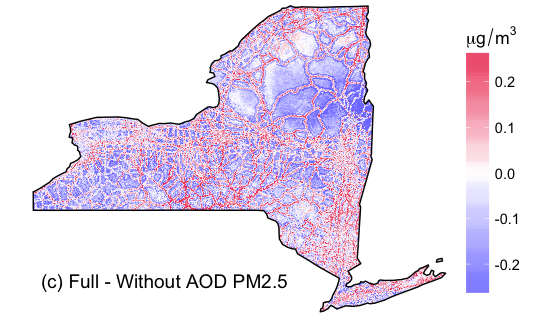
\includegraphics[width=0.7\textwidth]{img/no_aod.png}
    \caption{Spatial differences between full-model and no-AOD PM\tsub{2.5} in the snow season of 2015 (full-model minus no-AOD PM\tsub{2.5})}
    \label{fig:noaod}
\end{figure}

\begin{figure}[H]
    \centering
    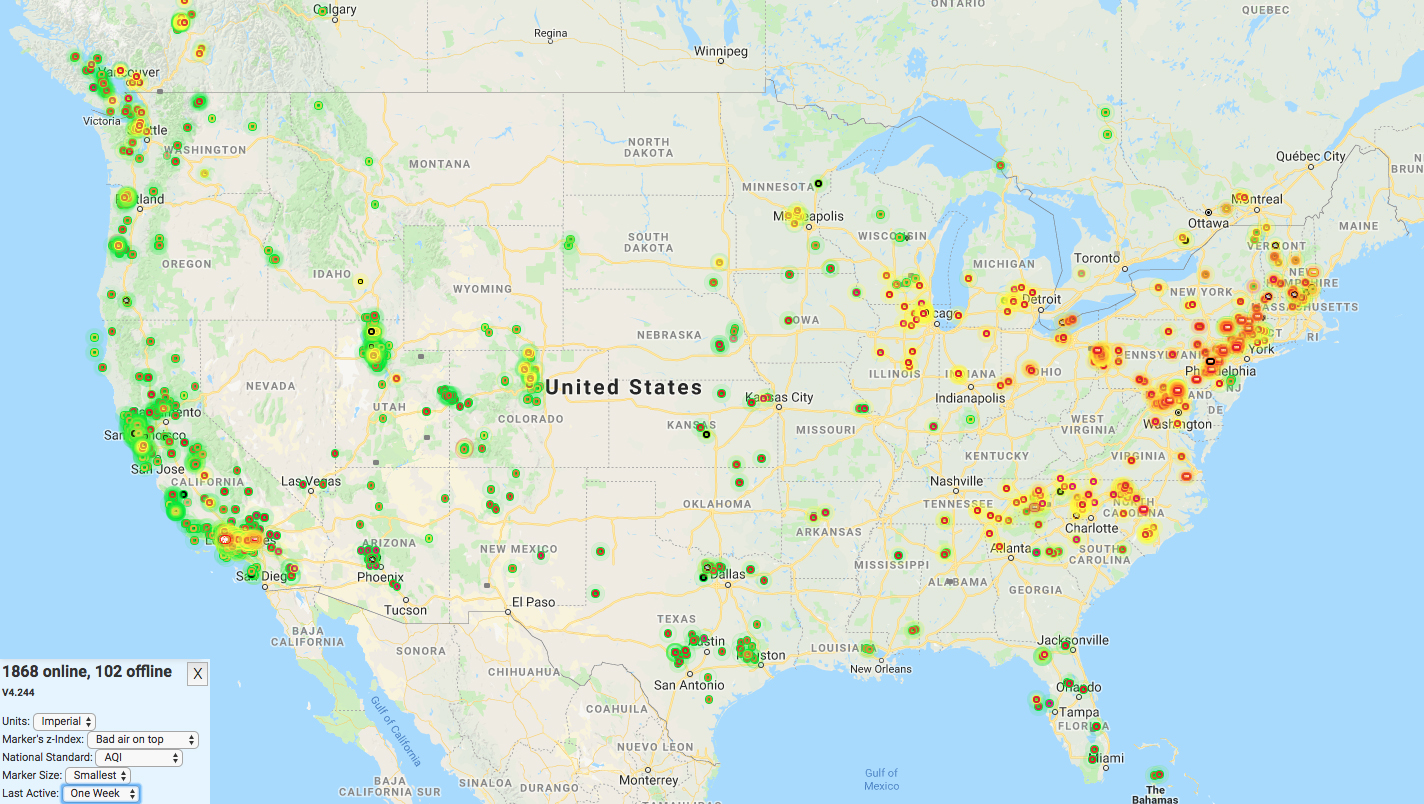
\includegraphics[width=0.9\textwidth]{img/purpleair.jpg}
    \caption{The distribution of PurpleAir low-cost sensors in the United States (Jun 19th, 2018)}
    \label{fig:pa}
\end{figure}

% ----------- References ----------- %
\newpage
\bibliographystyle{unsrtnat}
\bibliography{references}

\end{document}
